% SPDX-License-Identifier: CC-BY-4.0
%
% Copyright (c) 2023 Nelson Vieira
%
% @author Nelson Vieira <nelson0.vieira@gmail.com>
% @license CC-BY-4.0 <https://creativecommons.org/licenses/by/4.0/legalcode.txt>
\section{Methodology}

The overall work will be comprised of two phases which will be described
in the following paragraphs. Phase one mainly described throughout this
paper, focuses on collecting the state of the art in terms of the most relevant
topics, from which main privacy concepts were selected to be explored in
the stage 1 of Phase 2 with the preparation of a questionnaire to collect
user perceptions regarding privacy and topics collected in the systematic
literature review. The second stage of Phase 2 consists in developing an
application, partially based on the information generated by the survey,
that can identify what sort of devices are around, what kind of data is
gathered by these devices, present privacy options to the user when available,
and what can be done to prevent undesirable data from being collected.
\par
The Phase 1 Systematic Literature Review gathered the most relevant papers
discussing methodologies and techniques for the protection of users' privacy
data with special focus on IoT systems. For this SLR, this paper considered
focusing only on papers from the last 12 years, from 2010 until 2022, since
papers before then become out of date with the evolution of technology.
In this SLR, it was reviewed 54 papers published in top computer science,
security, privacy and software engineering outlets.

This paper followed Keshav's three-pass approach \cite{KeshavHow} when choosing
which papers to read fully and which ones to ignore, first the title would
be read, then the abstract, the introduction and conclusion and briefly
skim the rest of the paper and then decide if it was worth reading any further,
the focal point in this phase was answering the following question: does
the paper present a new methodology or interesting angle to tackle users'
privacy concerns? Only then the document would be read in its entirety while
ignoring any tables, figures, images or graphs. If the paper failed to present
any interesting idea, approach, or technique it would be discarded, but
if not, it would be read carefully from the beginning again in order to
fully understand what it presents. Having collected the major findings,
this work then aims to conduct a throughout study split in several stages
and around the specific research questions which will be explored in each
phase. For that matter, the research questions listed are:

\vspace{5mm}
\textbf{Phase 1:} \\
% \vfill

\textbf{RQ1:} What approaches are being considered for privacy issues in
IoT in the currently available literature?

\textbf{RQ2:} What are user perceptions on online privacy? \\

% \vspace{5mm}
\textbf{Phase 2:} \\
% \vfill

\textbf{RQ3:}
% What IoT-related tools are available that empower users to
% protect their privacy rights? OR
How to empower users to protect their privacy rights?

\textbf{RQ4:} What issues are prevalent in IoT that make it difficult to
address privacy and security problems?
\vspace{5mm}

The second phase will be evaluated on two stages, the first one consists
on doing a study on people's general privacy concerns, while using and interacting
with IoT devices. This study will abide on preparing a questionnaire to
assess general user's knowledge on privacy concepts, their habits and concerns,
their understanding of privacy rights, and what they do to safeguard those
rights. The goal of this study is to both understand the privacy paradox
and collect data on their proposal to address privacy issues with regard
to IoT devices.

% Having collected the major findings, this work then aims to conduct a throughout
% study split in several stages and around the following research questions:

% \textbf{RQ1:} What approaches are being considered for privacy issues in
% IoT in the currently available literature?

% \textbf{RQ2:} What IoT-related tools are available that empower users to
% protect their privacy rights? OR How to empower users to protect their privacy
% rights?

% \textbf{RQ3:} What issues are prevalent in IoT that make it difficult to
% address privacy and security problems?

% The proposed methodology is composed of two phases, the first phase consists
% on doing a study on people's general privacy concerns while using and interacting
% with IoT devices. This study will consist on preparing a questionnaire to
% assess general user's knowledge on privacy concepts, their habits and concerns,
% their understanding of privacy rights, and what they do to safeguard those
% rights. The goal of this study is to both understand the privacy paradox
% and collect data on their proposal to address privacy issues with regard
% to IoT devices. The second phase consists in developing an application, partially
% based on the information generated by the survey, that can identify what sort
% of devices are around, what kind of data is gathered by these devices, present
% privacy options to the user where available, and what can be done to prevent
% undesirable data from being collected.

% The second phase consists
% in doing an application that can detect IoT devices nearby the user with
% at least a 10 meters radius. The application should do the following when
% detecting a device:
% 1. it should show some information about the device;
% 2. it should categorize the device;
% 3. it should provide the user with privacy options, if the device allows the
% user to decline data harvesting.
% This application at first sight might appear to be a mere privacy assistant
% but it's not, because IoT assistants merely choose what privacy options the
% user first sets and maintains it for every other application that the user
% might use. The proposed app doesn't have the objective to conform to the user's
% preferred privacy choices, it merely informs the user about nearby IoT devices
% and can provide the user with privacy options. But the main objective is creating
% awareness in individuals about the various devices that are around and make
% the user questions their choices.

\subsection{Stage 1: User perceptions}

This study aims to understand people's perception of IoT and their privacy
practices online. It also serves to demystify the privacy paradox and also
to help provide a solution to the privacy issue in IoT. The questionnaire
consists of 92 questions divided into 7 sections to access users' knowledge,
it follows a kind of narrative, the first section being general privacy
questions then about the predisposition to data sharing, to concerns with
privacy then about daily digital routines, then about profile identification,
and then about IoT general knowledge before a section about non-identifiable
demographic data. The scale that is used in the questionnaire is based on
the work of Philip K. Masur \cite{masur2018situational}. Great care is taken
when it comes to this survey's data collection, in order to not identify
any individual or group of individuals, for instance, when it comes to differential
privacy, any data that might identify someone will not be disclosed, even
though the data might suffer from some inaccuracy because of this.

This survey was partially based in a study done in the Philippines by the
government in the context of their privacy act of 2012 \cite{Philippine2022Conduct},
this was the second survey done on the country's population. It was also
inspired by Alves's master's thesis \cite{alves2021}, which was about citizen's
perception about privacy in the wake of GDPR.

This survey was done through the internet, it was created in Google Forms,
this way it is guaranteed to reach the most people possible, besides Google
Forms itself, it will be used other online venues for distribution and even
printing.

Foram usados vários serviços de divulgação de questionários online
para angariar participantes, todos os serviços usados foram à base
da boa vontade dos participantes, portanto não houve qualquer incentivo
financeiros para o preenchimento do questionário. A maior parte dos serviços
usados são do tipo software as a service (SaaS) e baseiam-se em créditos
pelo preenchimento de outros questionários disponíveis nas plataformas,
isto torna o processo de adquirir participantes muito tedioso, pois
é necessário preencher muitos questionários para conseguir um número
razoável de participantes (pelo menos 400 a 500 participantes). Fazer a
divulgação do questionário desta forma não acarreta qualquer custo adicional,
mas pode fazer com que os resultados obtidos desta forma possam não
ser os mais honestos possíveis, pois alguns participantes podem estar
a preencher este questionário e forma rápida só para também conseguirem
angariar o número de participantes para os questionários deles próprios,
contudo também não há forma de garantir que caso este questionário fosse
realizado com algum incentivo financeiro que os participantes preenchessem
da forma mais honesta possível. Para além da divulgação pelos vários serviços,
também foram usadas as redes sociais e foi divulgado pessoalmente para família e
amigos. Uma forma possível de divulgação seria pessoalmente, de casa em casa, mas
seria esta seria uma forma muito lenta de conseguir respostas e também as
pessoas poderiam se sentir obrigadas a responder e desta forma não seria
muito ético, para além de as respostas poderem ter sido respondidas de uma
forma pouco honesta.

O questionário esteve disponível para preenchimento até ao dia 30 de Abril de 2023,
e durante o tempo em que esteve aberto foi possível obter respostas de x participantes.


\subsection{Stage 2: Study in Context, an Application}

This work proposes an application that gives users information about IoT
devices in their surroundings like the type of information these devices
collect and what privacy options are available. This application will be
developed for mobile phones because it is the most used device that people
take everywhere they go, and because the application will use georeferencing
to show the location of the IoT devices. The main objective of this application
is to give users another option in order to protect their private data.
The application will show the geolocation of the IoT devices, what type
of device it is, what type of data is being collect by the device. The application
will not detect the devices by itself, this will be done by the users themselves,
in the first few iterations of this application it was proposed that the
application itself would detect the devices and would categorize what type
of device it was and what type of data it was collecting but it was discovered
that this approach was too complex and so it was not feasible to do with
the constraints of this paper. The application will be developed with Flutter,
other options could be React Native or a progressive web application, but
Flutter uses ahead of time and just in time compilation with Dart as it
is programming language while React Native uses the Javascript programming
language that was never created for mobile programming so it uses a bridge
to convert Javascript to native components for Android or iOS. Flutter has
better performance and as such it is the chosen framework for this application.

Types of data:
Health
Visual
Audio
Presence (if user is nearby)
Location (precise location of user)
Biometrics
Environment
Unique identification (with the help of other means)

Infomation to be added to the app:
What is the purpose of the data collection
Who can access the data
For how long is it stored
Can the data identify anyone
What is done with this data

\section{Current Stage of the Work}

The preliminary results of the study, based on 10 responses, show that everyone
agrees that privacy is important to them and some people know that they
should not share their personal information with anyone they do not trust
(like clicking on random urls or using unprotected websites/software), but
most of them think that privacy and security are the same concept, most
respondents also do not read privacy notices but accept them to access the
information they want to get to, most respondents use their devices mostly
to access social networks and for work, when it comes to IoT, there is a
dissonance between knowing the term and using devices like smart watches
or RFID enabled devices, from the respondents that answered yes to using
IoT devices most use because of work. It is also noted that most respondent
have a background in engineering, so the responses are skewed. As a result,
the survey will remain open to gather a larger number of responses and participants
for more significant results and generalizations.

\begin{table}[ht]
\centering
\begin{adjustbox}{width=0.5\textwidth}
\small
\noindent\begin{tabular}{p{0.17\textwidth}*{20}{|p{0.01\textwidth}}|}
\hline
\multicolumn{0}{|c|}{Work plan}
    & \multicolumn{4}{c|}{January}
    & \multicolumn{4}{c|}{February}
    & \multicolumn{4}{c|}{March}
    & \multicolumn{4}{c|}{April}
    & \multicolumn{4}{c|}{May}
    \\
\hline
\hline
\multicolumn{0}{|l|}{Week}
    & 1 & 2 & 3 & 4 & 1 & 2 & 3 & 4& 1 & 2 & 3 & 4& 1 & 2 & 3 & 4& 1 & 2 & 3 & 4 \\
\hline
% using the on macro to fill in twenty cells as `on'
\multicolumn{0}{|l|}{Discovery and planning}
    & \cellcolor[cmyk]{1,1,0,0}&&&& &&&& &&&& &&&&&&& \\
\hline
\multicolumn{0}{|l|}{Research enquiry}
    & \cellcolor[cmyk]{1,1,0,0} & \cellcolor[cmyk]{1,1,0,0} & \cellcolor[cmyk]{1,1,0,0} & \cellcolor[cmyk]{1,1,0,0} & \cellcolor[cmyk]{1,1,0,0} & \cellcolor[cmyk]{1,1,0,0} & \cellcolor[cmyk]{1,1,0,0} & \cellcolor[cmyk]{1,1,0,0} & \cellcolor[cmyk]{1,1,0,0} & \cellcolor[cmyk]{1,1,0,0} & \cellcolor[cmyk]{1,1,0,0} & \cellcolor[cmyk]{1,1,0,0} &&&& &&&& \\
\hline
\multicolumn{0}{|l|}{State of the art}
    & \cellcolor[cmyk]{1,1,0,0} & \cellcolor[cmyk]{1,1,0,0} & \cellcolor[cmyk]{1,1,0,0} & \cellcolor[cmyk]{1,1,0,0} & \cellcolor[cmyk]{1,1,0,0} & \cellcolor[cmyk]{1,1,0,0} & \cellcolor[cmyk]{1,1,0,0} & \cellcolor[cmyk]{1,1,0,0} &&&& &&&& &&&& \\
\hline
\multicolumn{0}{|l|}{Project requirements}
    & \cellcolor[cmyk]{1,1,0,0} & \cellcolor[cmyk]{1,1,0,0} & \cellcolor[cmyk]{1,1,0,0} & \cellcolor[cmyk]{1,1,0,0} &&&& &&&& &&&& &&&& \\
\hline
\multicolumn{0}{|l|}{Wireframes and user stories}
    &&&& & \cellcolor[cmyk]{1,1,0,0} & \cellcolor[cmyk]{1,1,0,0} & \cellcolor[cmyk]{1,1,0,0} & \cellcolor[cmyk]{1,1,0,0} &&&& &&&& &&&& \\
\hline
\multicolumn{0}{|l|}{Prototyping and refinement}
    &&&&&& && \cellcolor[cmyk]{1,1,0,0} & \cellcolor[cmyk]{1,1,0,0} & \cellcolor[cmyk]{1,1,0,0} & \cellcolor[cmyk]{1,1,0,0} &&&& &&&& &  \\
\hline
\multicolumn{0}{|l|}{Development}
    &&&& &&&& & \cellcolor[cmyk]{1,1,0,0} & \cellcolor[cmyk]{1,1,0,0} & \cellcolor[cmyk]{1,1,0,0} & \cellcolor[cmyk]{1,1,0,0} & \cellcolor[cmyk]{1,1,0,0} & \cellcolor[cmyk]{1,1,0,0} & \cellcolor[cmyk]{1,1,0,0} & \cellcolor[cmyk]{1,1,0,0} & \cellcolor[cmyk]{1,1,0,0} & \cellcolor[cmyk]{1,1,0,0} & \cellcolor[cmyk]{1,1,0,0} & \cellcolor[cmyk]{1,1,0,0} \\
\hline
\multicolumn{0}{|l|}{Tests and iterations}
    &&&& &&&& &&& & \cellcolor[cmyk]{1,1,0,0} & \cellcolor[cmyk]{1,1,0,0} & \cellcolor[cmyk]{1,1,0,0} & \cellcolor[cmyk]{1,1,0,0} & \cellcolor[cmyk]{1,1,0,0} &&&&  \\
\hline
\multicolumn{0}{|l|}{Release and documentation}
    &&&& &&&& &&&& &&&& & \cellcolor[cmyk]{1,1,0,0} & \cellcolor[cmyk]{1,1,0,0} & \cellcolor[cmyk]{1,1,0,0} & \cellcolor[cmyk]{1,1,0,0} \\
\hline
\end{tabular}
\end{adjustbox}
\vspace{1em}
\caption{Work plan timeline}
\label{workchart}
\end{table}

As can be seen in Table \ref{workchart}, the first months will involve the
design of the application and the enquiry of the study followed by the development
of the application and the synthesis of the study, and finally testing and
refinement of the application. Because of the exploratory nature of this
work the application might suffer alterations to the design, specially in
the testing stage, and also depending on the results of the study.

\section{Prototype}

\begin{figure}
    \begin{center}
        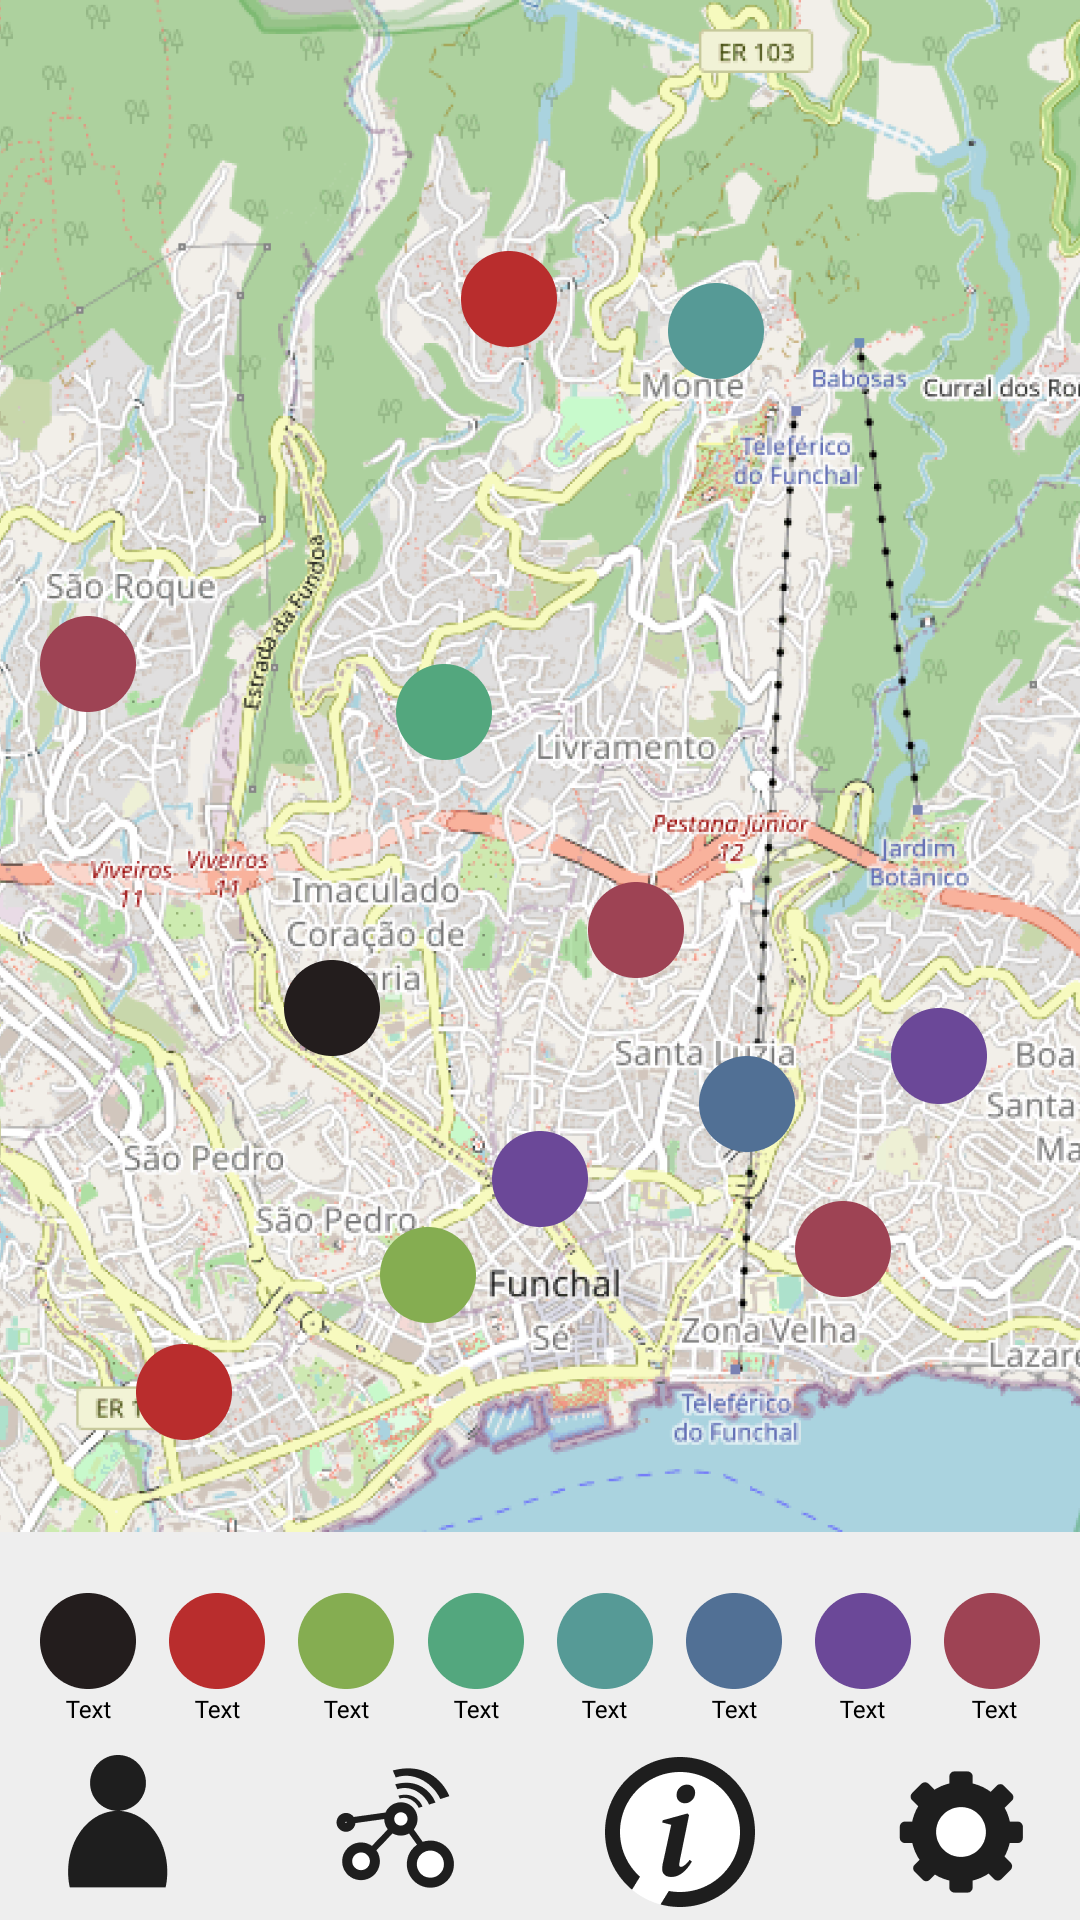
\includegraphics[width=130pt]{../assets/images/low_homepage.png}
        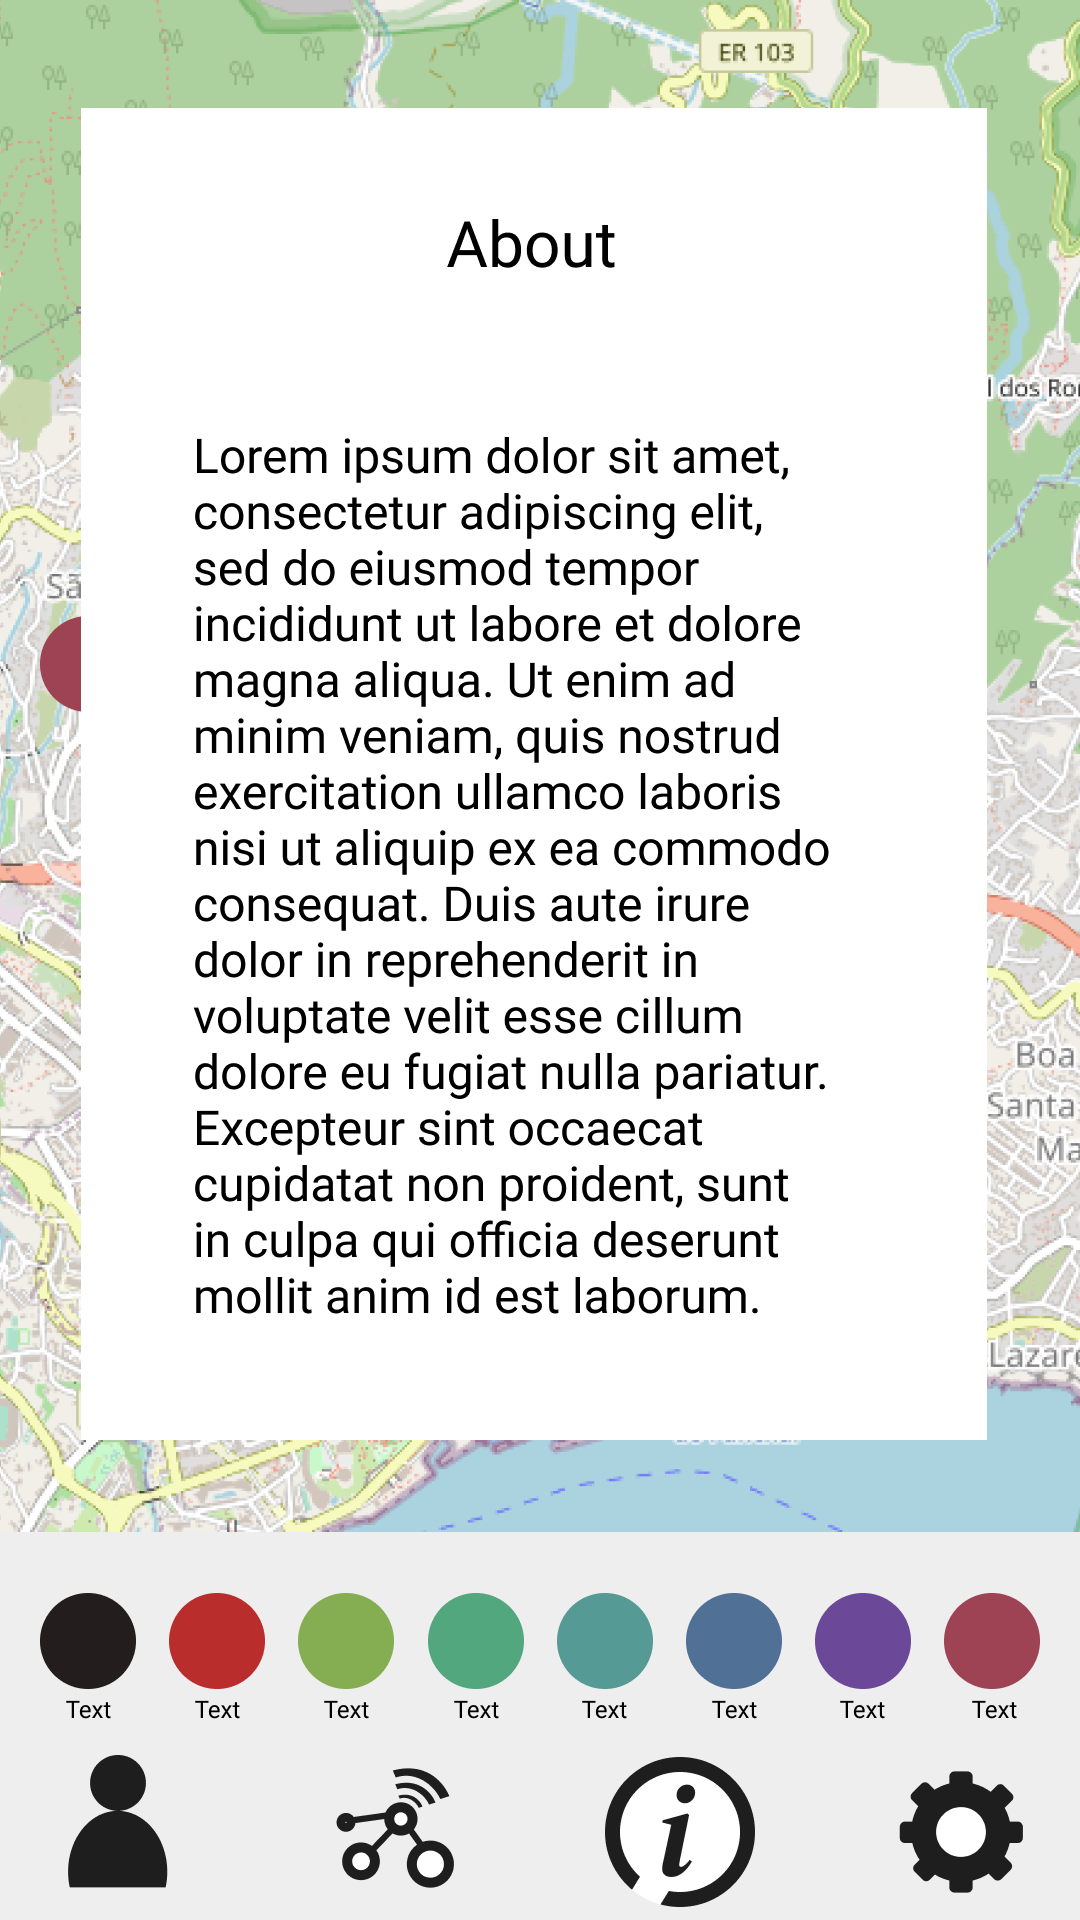
\includegraphics[width=130pt]{../assets/images/low_about.png}
        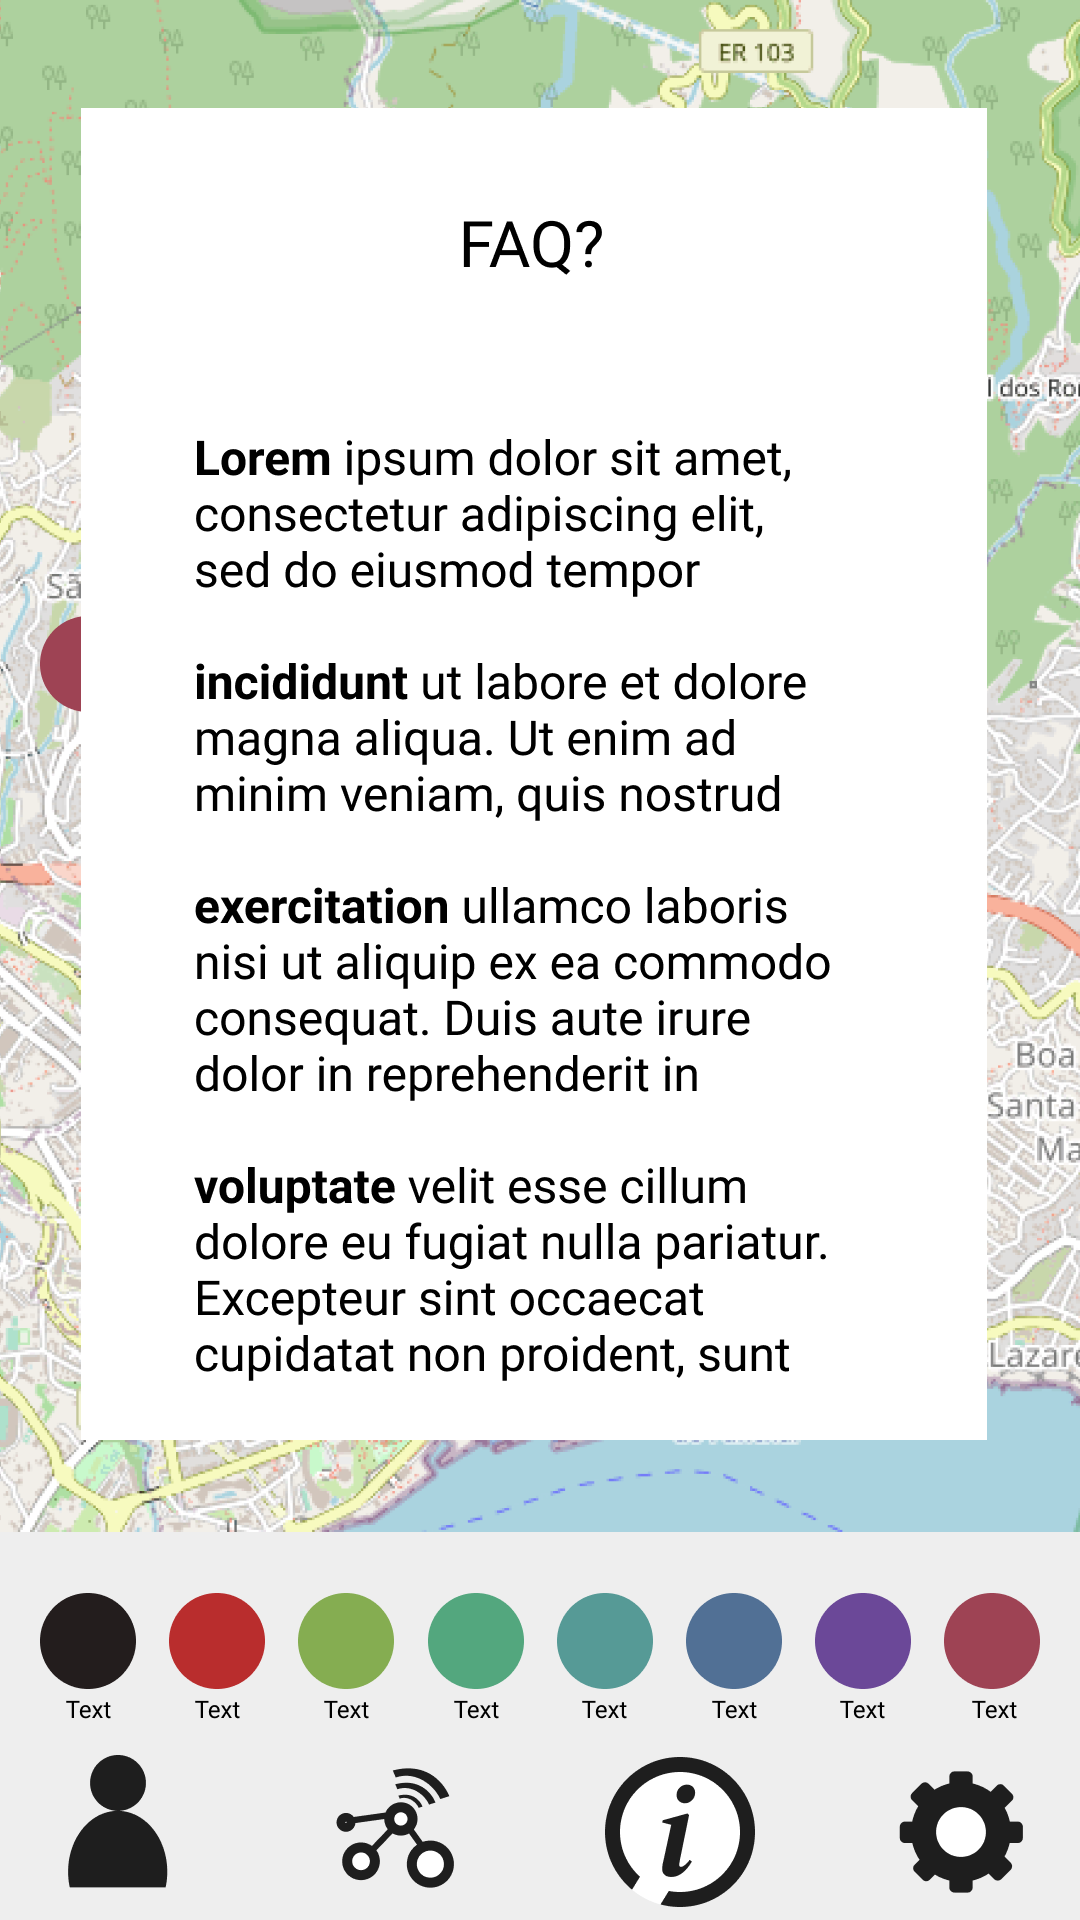
\includegraphics[width=130pt]{../assets/images/low_more_info.png}
        \caption{Low level prototype of homepage, about and FAQ pages.}
        \label{fig:lowlevelprototype}
    \end{center}
\end{figure}

\begin{figure}
    \begin{center}
        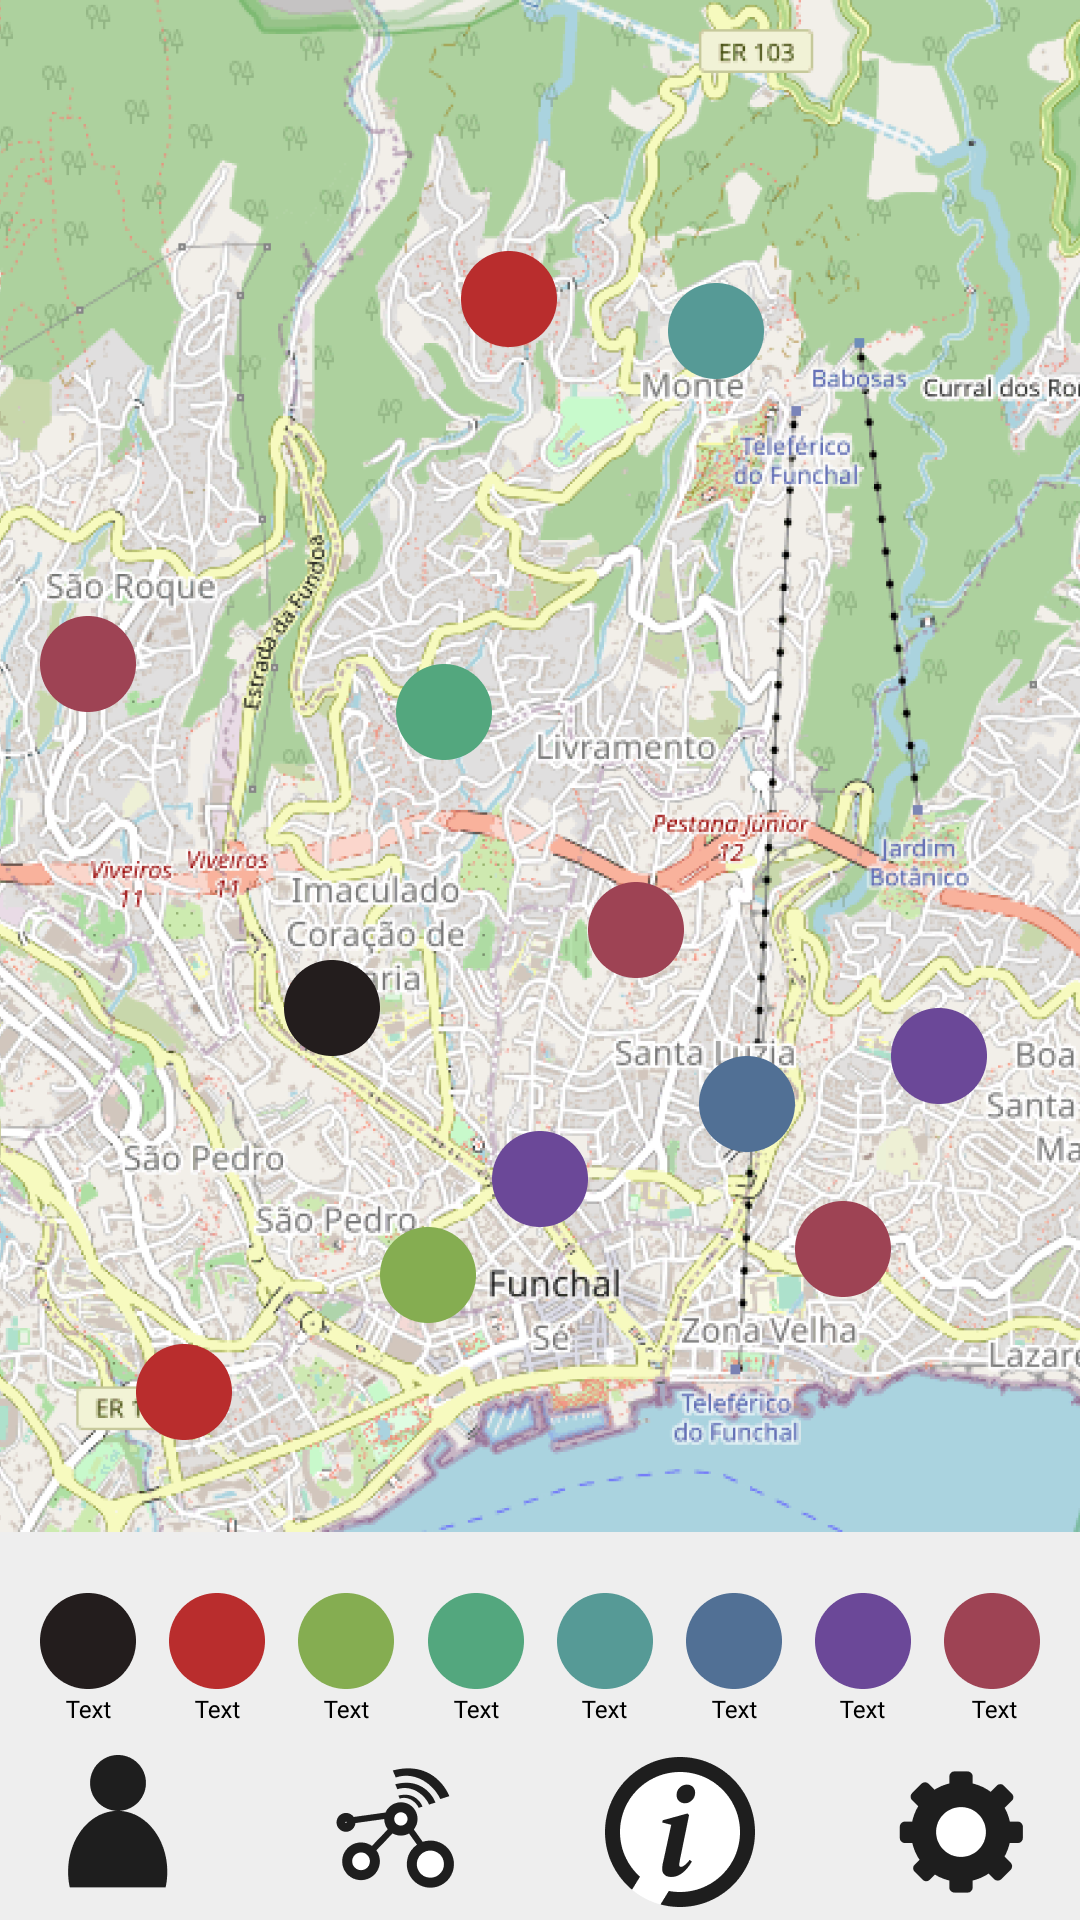
\includegraphics[width=130pt]{../assets/images/low_homepage.png}
        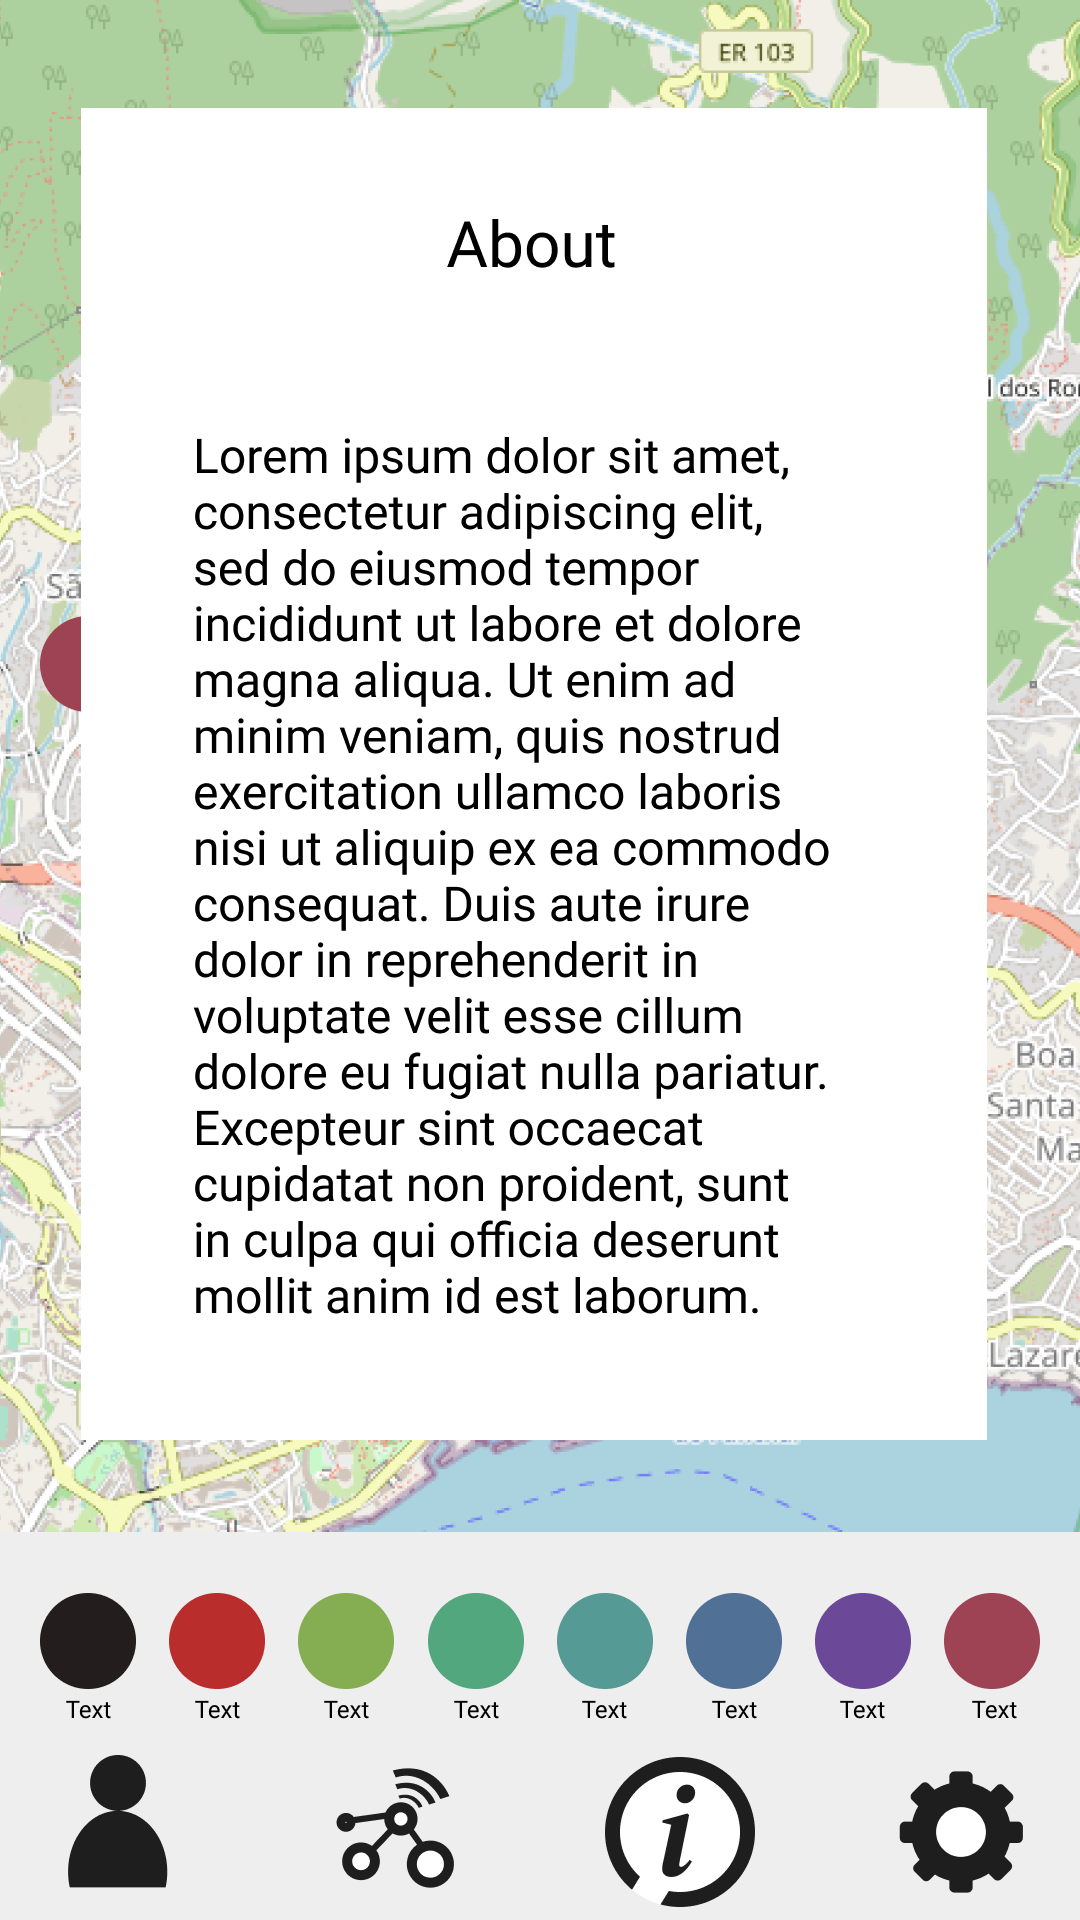
\includegraphics[width=130pt]{../assets/images/low_about.png}
        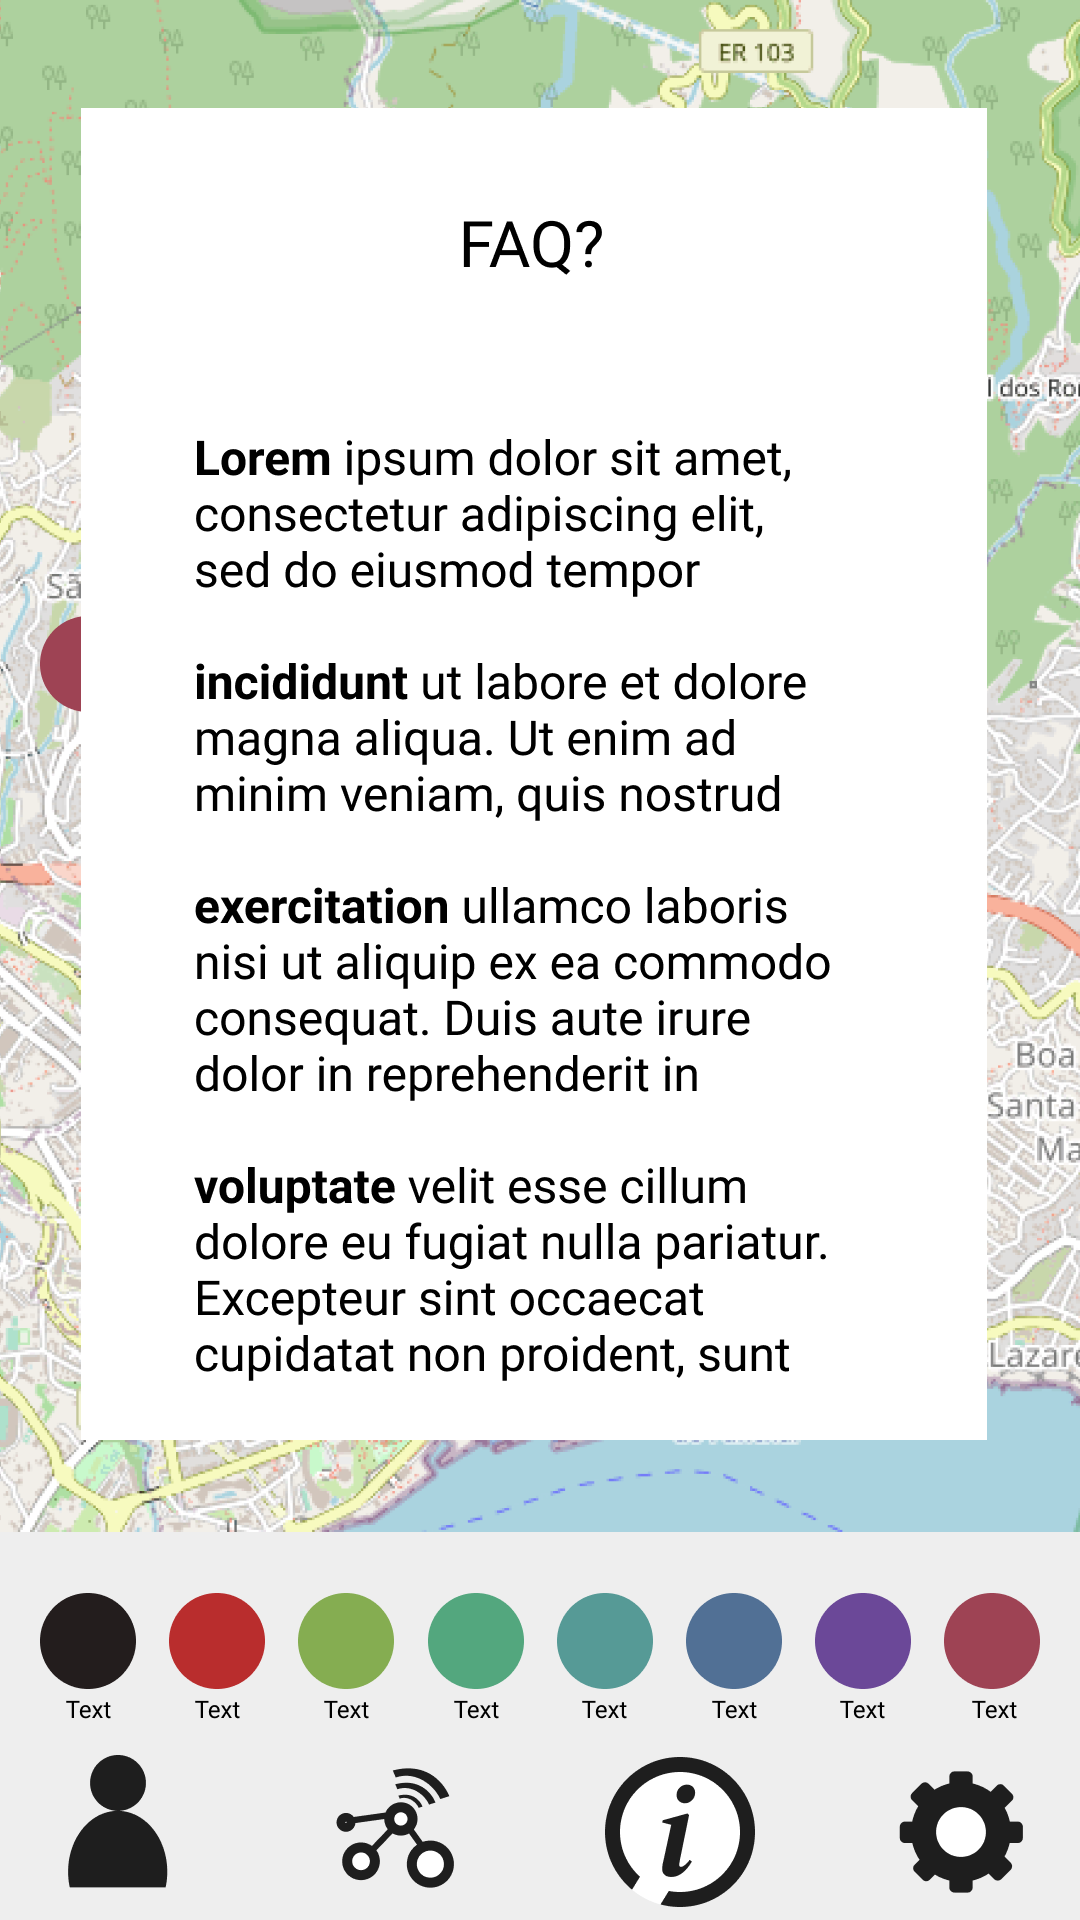
\includegraphics[width=130pt]{../assets/images/low_more_info.png}
        \caption{Medium level prototype of homepage, about and FAQ pages.}
        \label{fig:mediumlevelprototype}
    \end{center}
\end{figure}

\begin{figure}
    \begin{center}
        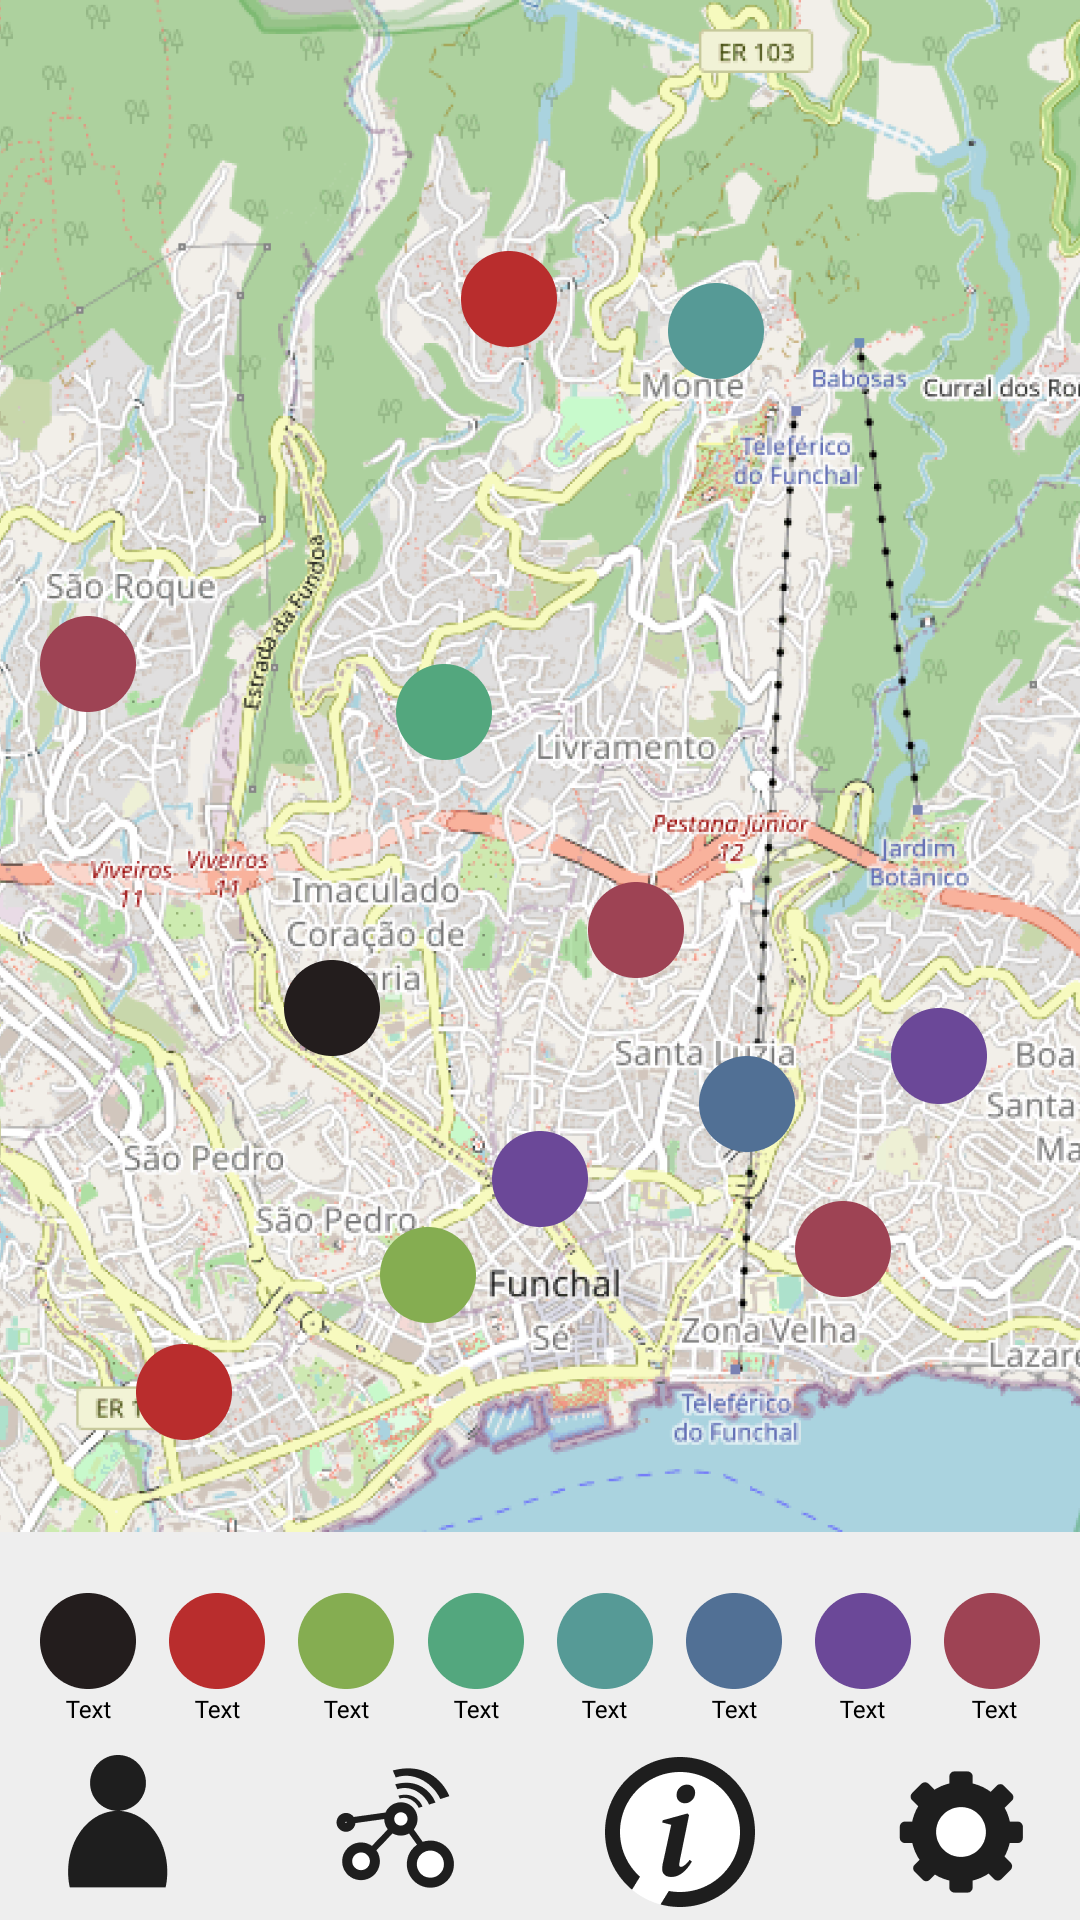
\includegraphics[width=130pt]{../assets/images/low_homepage.png}
        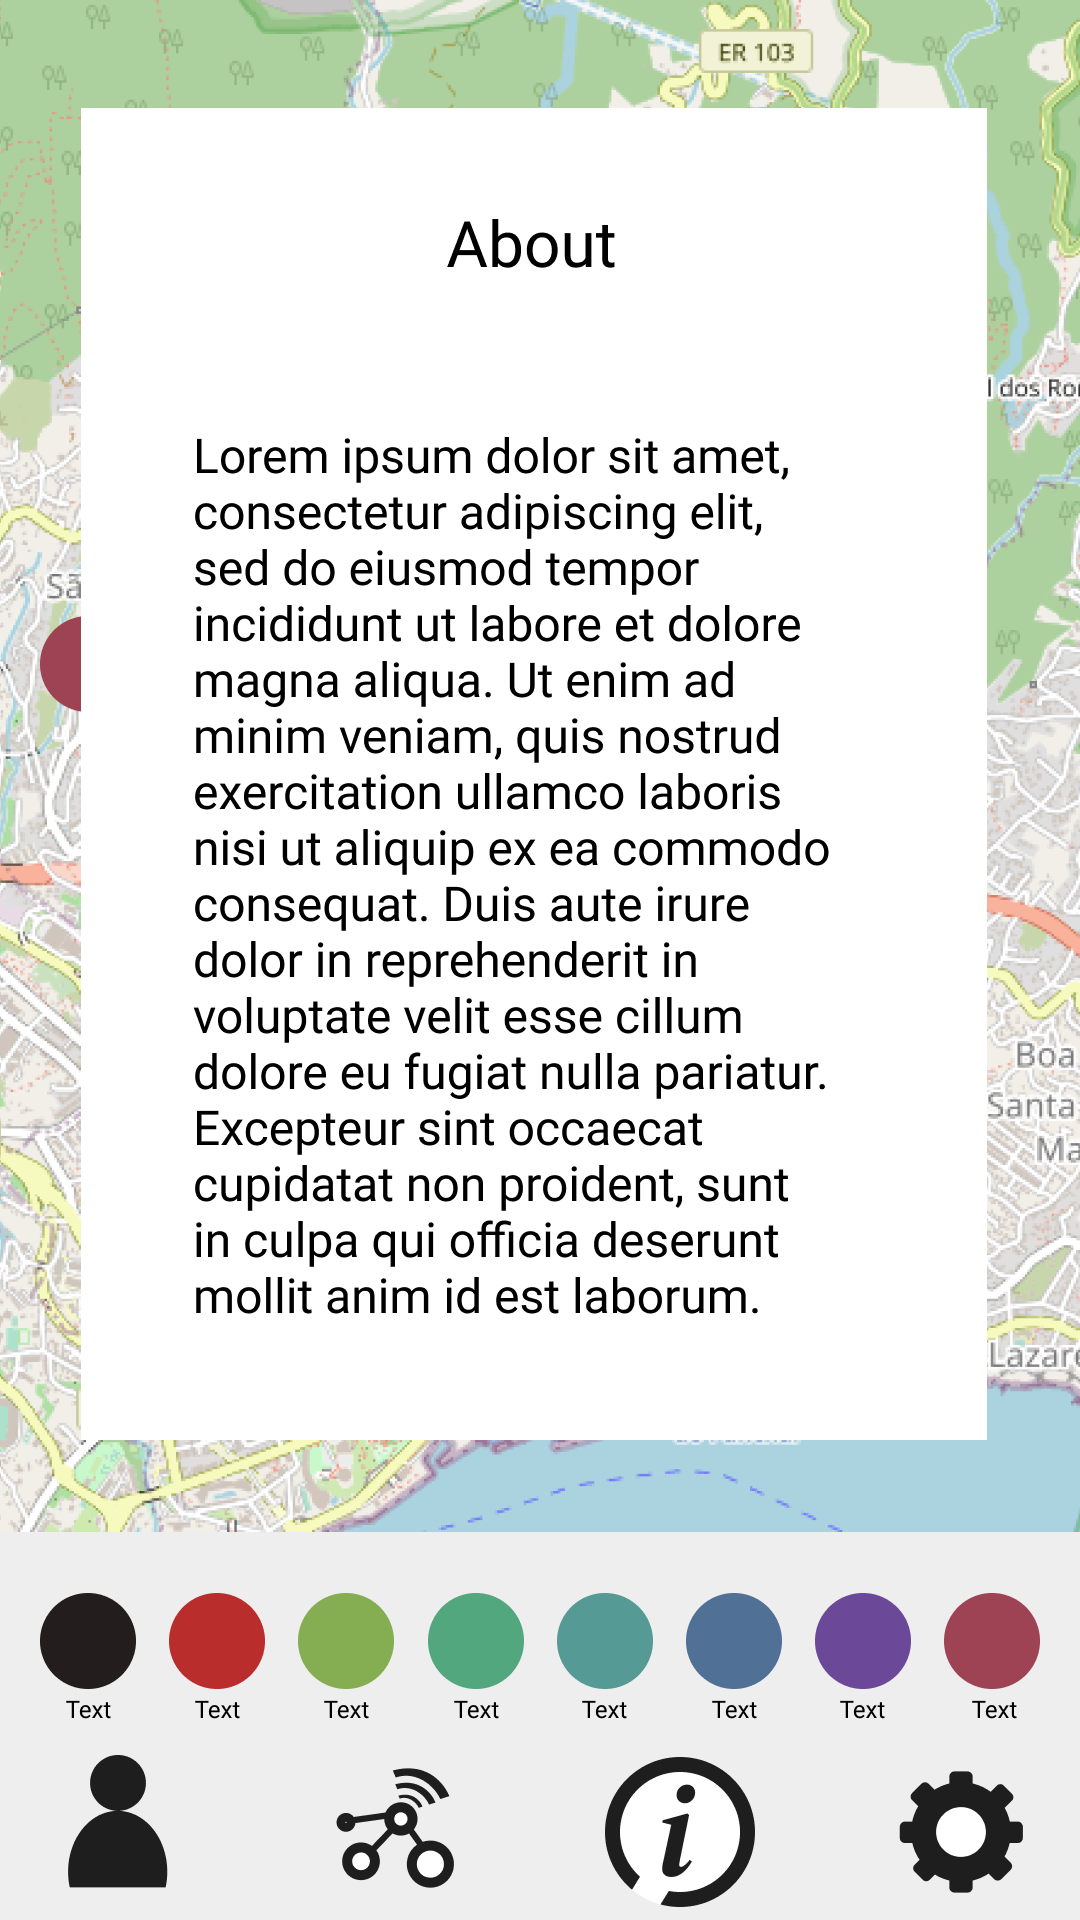
\includegraphics[width=130pt]{../assets/images/low_about.png}
        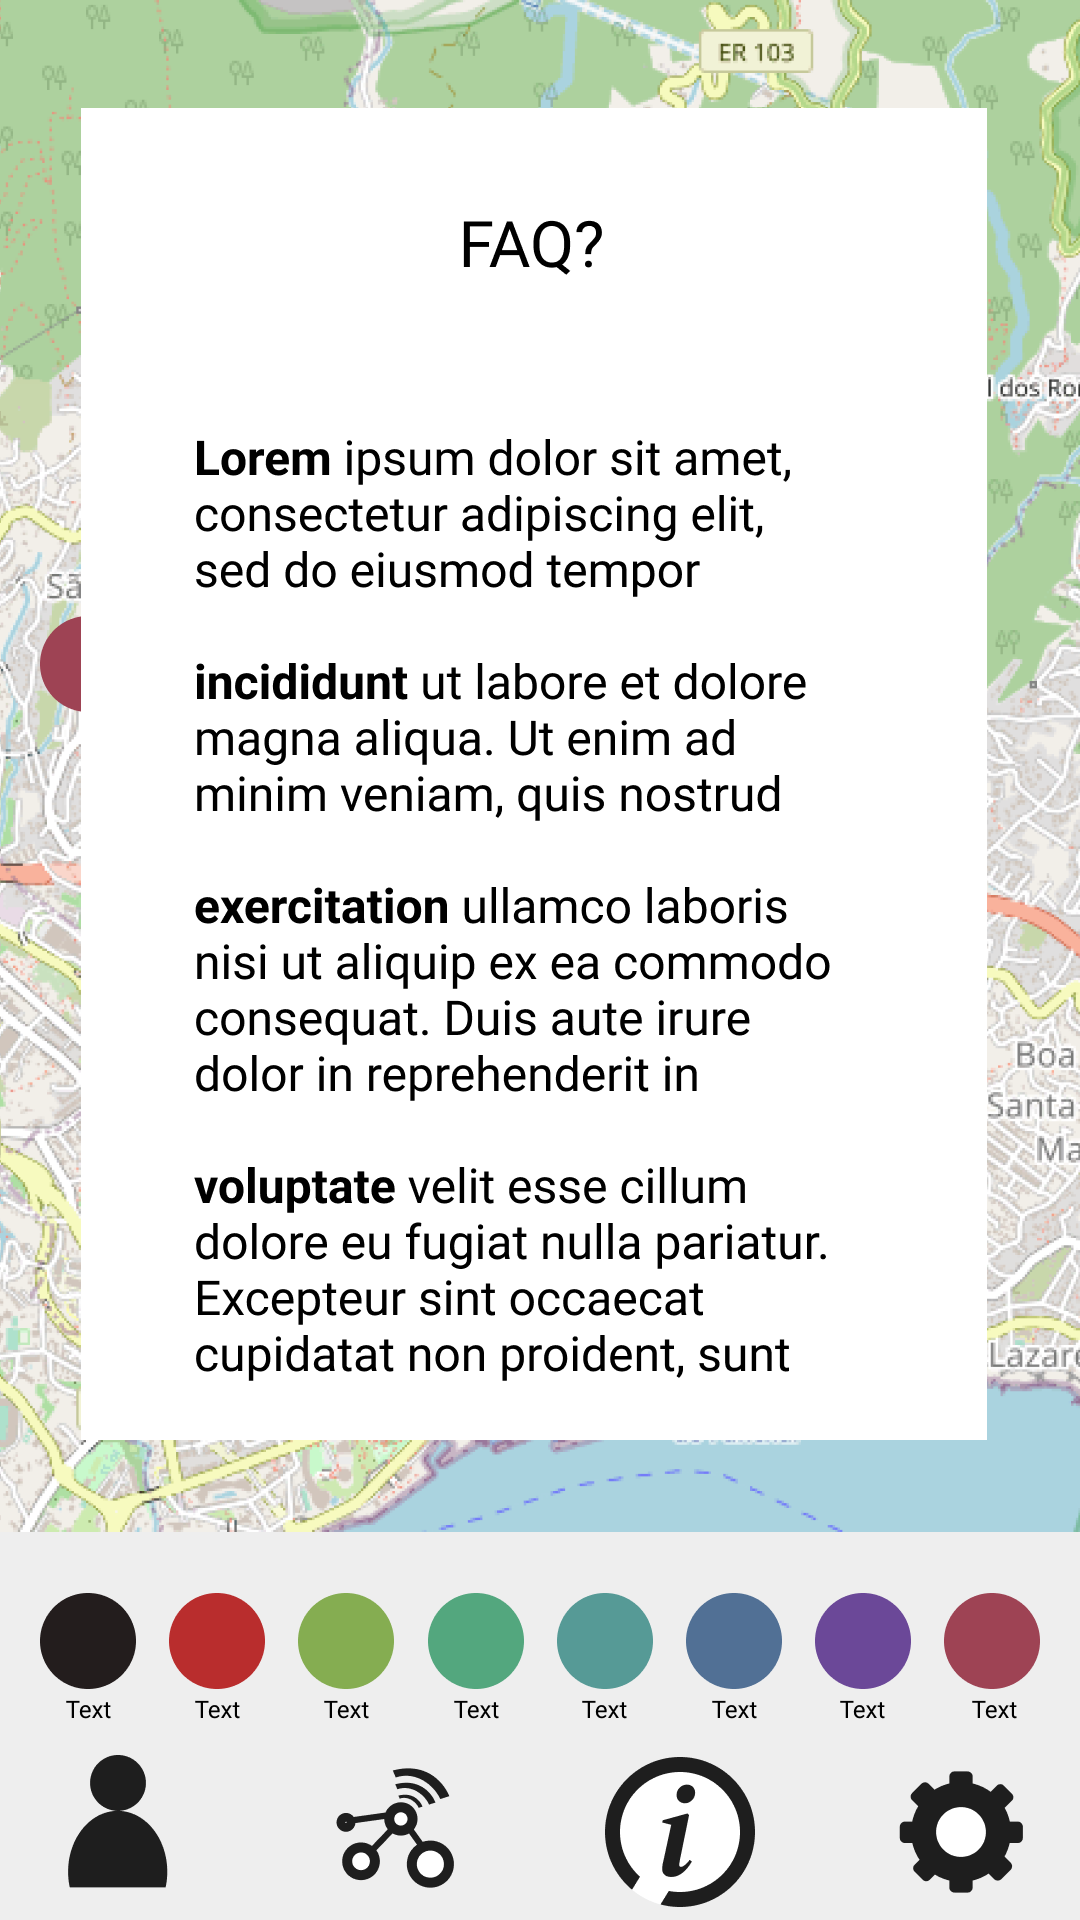
\includegraphics[width=130pt]{../assets/images/low_more_info.png}
        \caption{High level prototype of homepage, about and FAQ pages.}
        \label{fig:highlevelprototype}
    \end{center}
\end{figure}

\section{Challenges}

One of the most difficult points to accomplish in this thesis was the
questionnaire, not the fact of constructing the questionnaire but of
getting participants. Besides being difficult in itself to get a relatively
high number of participants of participants (a few hundred at least)
to be able to draw conclusions with any high degree of confidence, it was
difficult to get to get the potential participants interested in the topic
at hand, because although it seems that many people value their privacy very
highly and think they should protect it in practice they are not very
interested. This may even be because many people do not have much knowledge
about the Internet of Things, and thus feel that they cannot answer the
questionnaire because it is out of their field of knowledge, another
reason may be that the questionnaire seems a little long, because it
takes on average 15 to 20 minutes to answer, and despite being a topic
of interest the time investment in the questionnaire may be considered
too high. Another point to take into consideration regarding the low
number of participants is the way the questionnaire is written and how
it was advertised, i.e., a very formal or technical language may have
been used both in the construction of the questionnaire and in its
dissemination, and the fact that this is a very niche topic may have
"scared" possible participants. However, it should be noted that also
in the literature that has been carried out there is not a great focus
on conducting questionnaires and the ones that have been conducted have
not only focused on the Internet of Things and also have some monetary
incentive for the participants.

% Um dos pontos mais difíceis de realizar nesta tese foi o questionário,
% não o facto de construir o questionário mas sim de angariar participantes.
% Para além de ser difícil por si só conseguir ter um número de participantes
% relativamente alto (algumas centenas, 500 a 1000) para conseguirmos tirar
% conclusões com algum grau de confiança elevado, foi difícil de conseguir
% com que os possíveis participantes se interessassem no tópico em questão,
% pois apesar de parecer que muitas pessoas valorizem muito a sua privacidade
% e achem que devem a proteger na prática não se interessam muito. Isto até
% pode ser porque muitas pessoas não tenham muito conhecimento a nível da
% Internet of Things, e assim acharem que não conseguem responder ao questionário
% por ser fora do seu campo de conhecimento, outra razão pode o questionário
% parecer um pouco longo, pois demora em média 15 a 20 minutos para responder,
% e apesar de até ser um tópico de interesse o investimento de tempo no
% questionário pode ser considerado muito elevado. Outro ponto a ter em consideração
% em relação ao baixo número de participantes é a forma como o questionário
% está escrito e como este foi divulgado, isto é, pode ter sido usado
% uma linguagem muito formal ou técnica tanto na construção do mesmo como
% também na sua divulgação e juntado ao facto de este ser um tópico muito niche
% pode ter "assustando" possíveis participantes. Contudo é de notar que
% também na literatura que tem vindo a ser realizada não há um grande foco
% na realização de questionários e os que têm sido realizados não têm se
% focado somente na Internet of Things e têm também algum incentivo monetário
% para os participantes.
